\section{Kết quả và phân tích}

\subsection{Thông số dùng để mô phỏng}
Bảng~\ref{tab:params} tổng hợp các số liệu đầu vào được nhóm sử dụng để chạy mô phỏng và vẽ các đồ thị trong chương này.

\begin{table}[H]
\centering
\caption{Bộ thông số mặc định}
\label{tab:params}
\begin{tabular}{|c|l|c|c|}
\hline
\textbf{Ký hiệu} & \textbf{Đại lượng} & \textbf{Giá trị} & \textbf{Đơn vị} \\
\hline
$m$ & Khối lượng của vật & 1{,}0 & kg \\
$g$ & Gia tốc trọng trường & 9{,}81 & m/s$^2$ \\
$h$ & Hệ số cản của không khí & 0{,}5 & kg/s \\
$v_0$ & Vận tốc ném ban đầu & 50{,}0 & m/s \\
$t_{max}$ & Thời gian quan sát tối đa & 15{,}0 & s \\
$\alpha$ & Các góc ném khảo sát & 15, 30, 45, 60, 75 & độ \\
\hline
\end{tabular}
\end{table}


\subsection{Quỹ đạo ở các góc ném khác nhau}

Hình~\ref{fig:trajectories} vẽ lại đường bay của vật ở năm góc ném khác nhau. Bảng~\ref{tab:data} ghi lại các số liệu chi tiết tương ứng.

\begin{figure}[H]
\centering
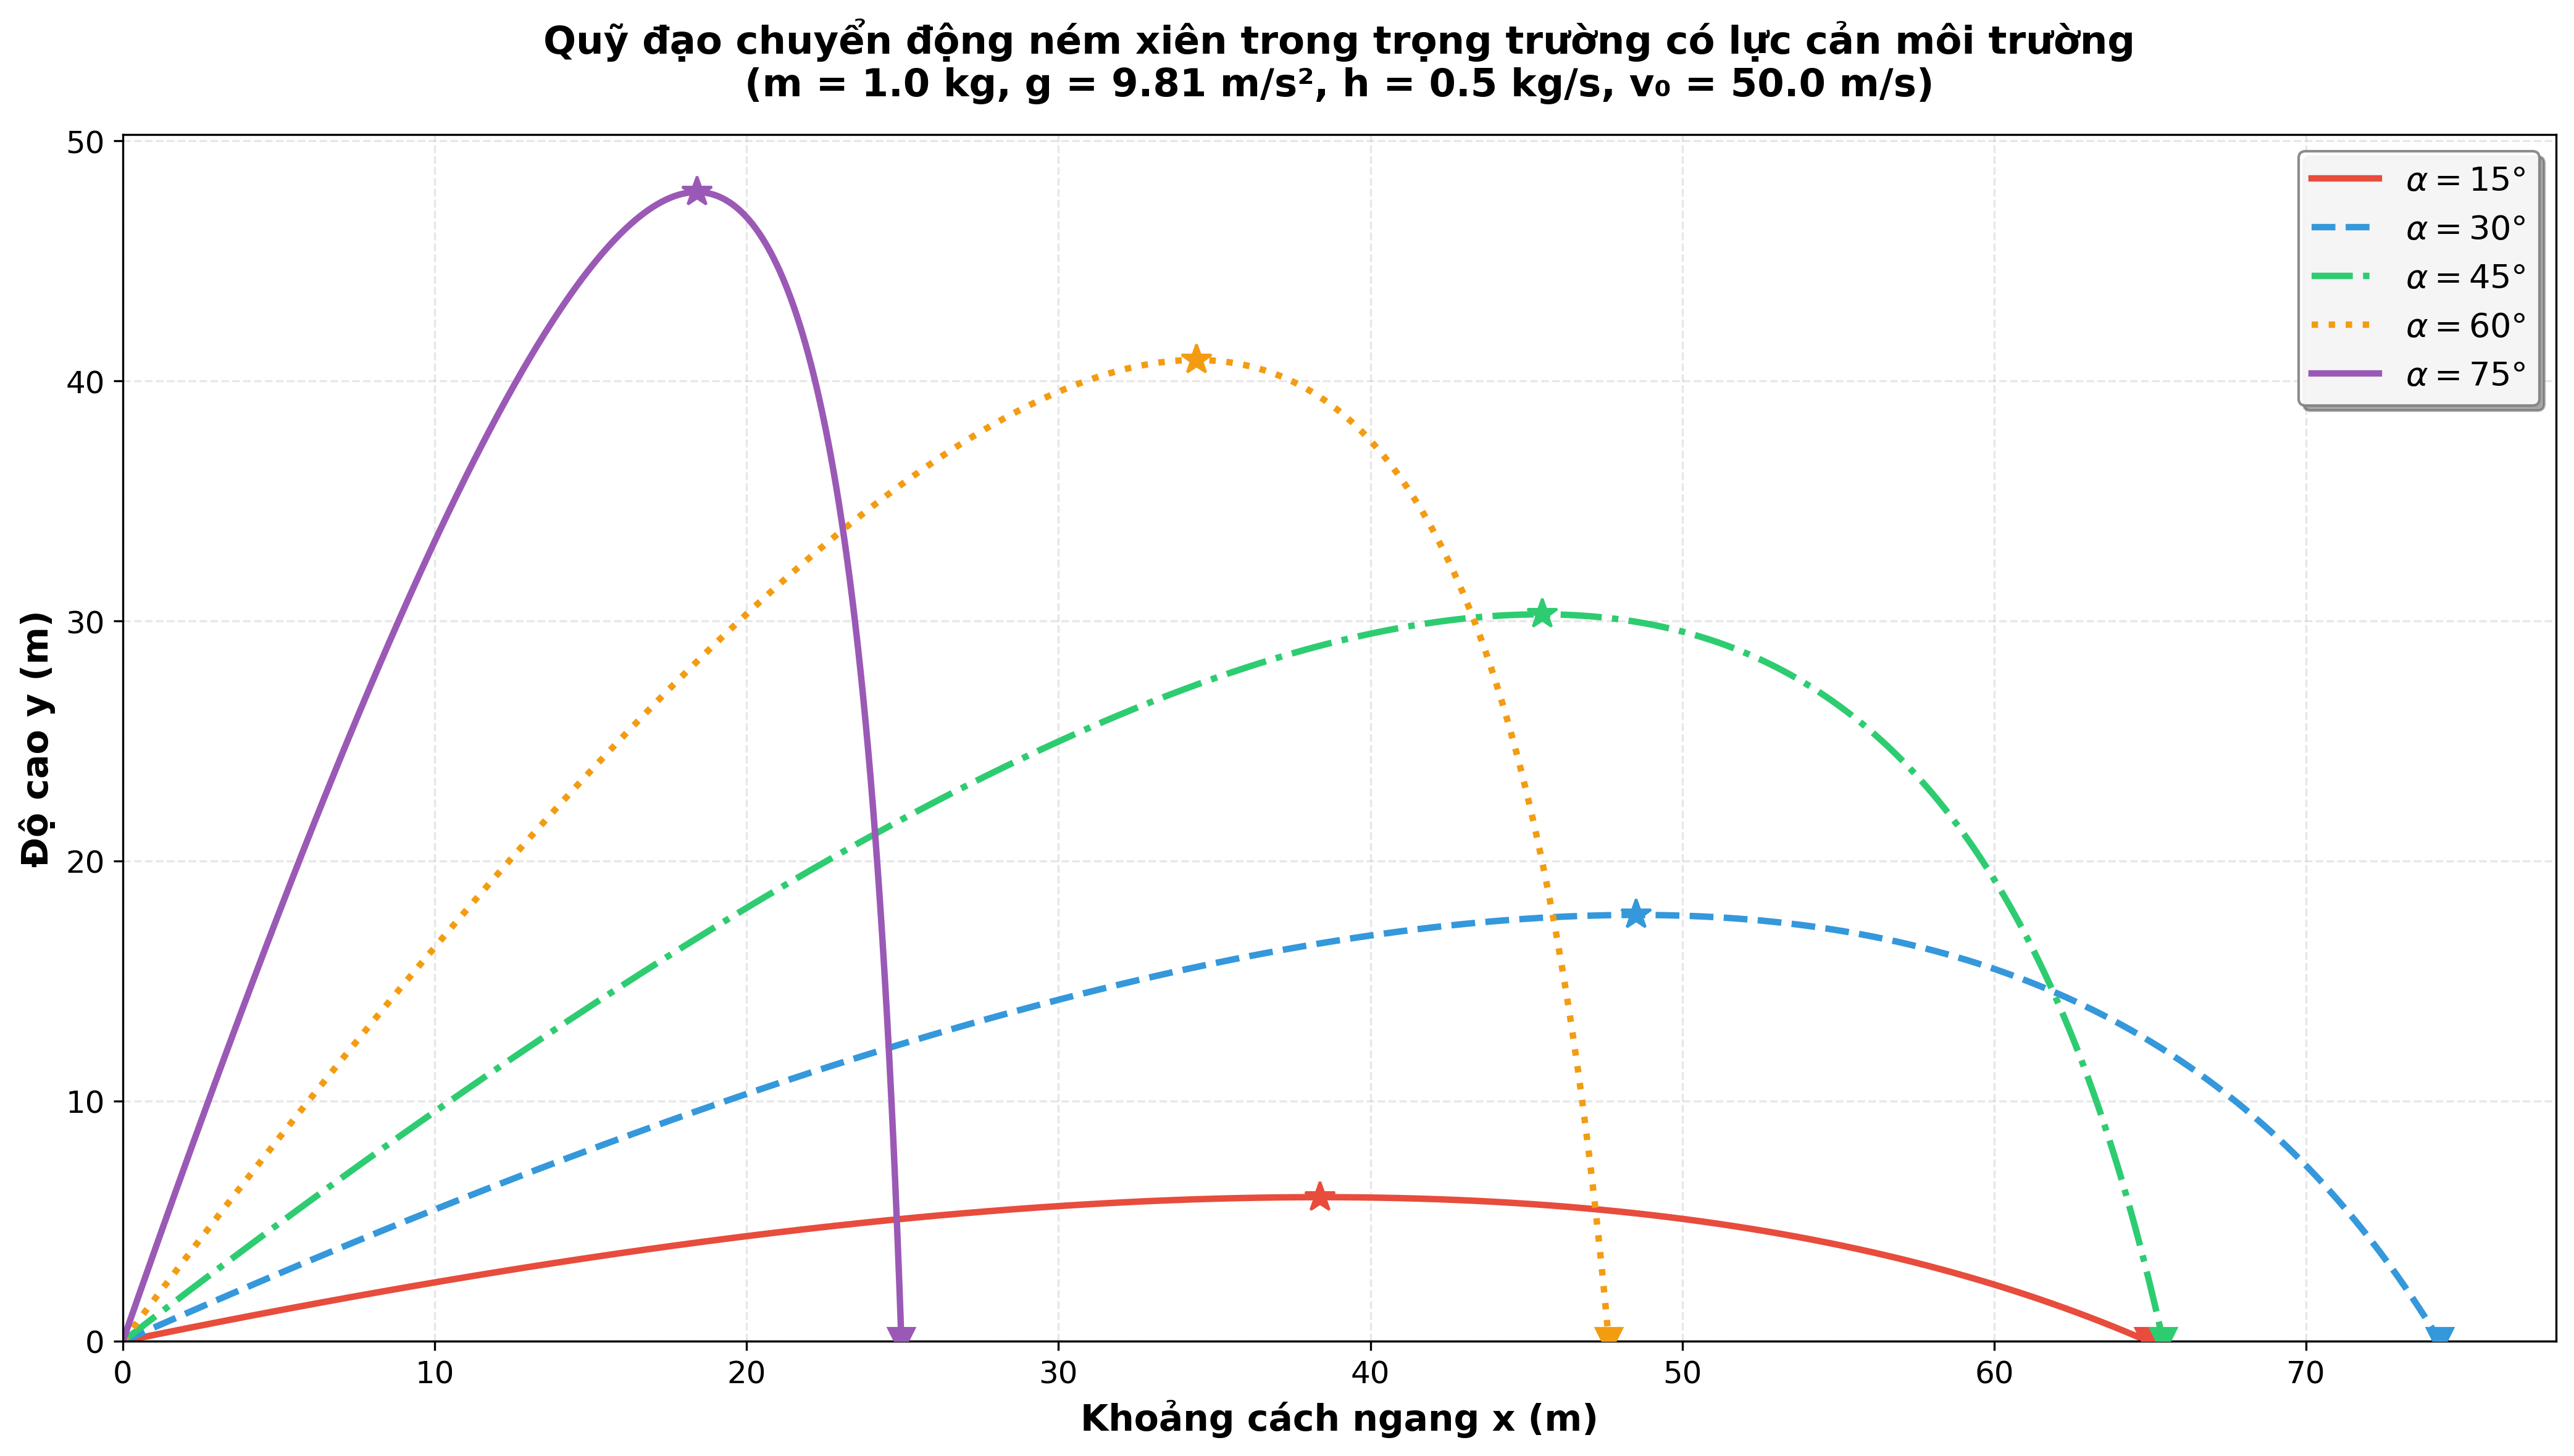
\includegraphics[width=\textwidth]{images/quy_dao_nem_xien.png}
\caption{Đường bay của vật khi có lực cản ($h = 0{,}5$ kg/s) ở các góc 15°, 30°, 45°, 60°, 75°. Dấu $\diamond$ là đỉnh cao nhất, dấu $\blacktriangledown$ là điểm rớt xuống đất.}
\label{fig:trajectories}
\end{figure}

\begin{table}[H]
\centering
\caption{Số liệu quỹ đạo ở năm góc ném ($h = 0{,}5$ kg/s)}
\label{tab:data}
\begin{tabular}{|c|c|c|c|c|c|}
\hline
$\alpha$ (°) & $v_{0x}$ (m/s) & $v_{0y}$ (m/s) & Tầm xa $R$ (m) & $H_{max}$ (m) & $T$ (s) \\
\hline
15 & 48{,}30 & 12{,}94 & 64{,}95 & 6{,}00 & 2{,}23 \\
30 & 43{,}30 & 25{,}00 & 74{,}29 & 17{,}76 & 3{,}90 \\
45 & 35{,}36 & 35{,}36 & 65{,}42 & 30{,}28 & 5{,}19 \\
60 & 25{,}00 & 43{,}30 & 47{,}65 & 40{,}88 & 6{,}11 \\
75 & 12{,}94 & 48{,}30 & 24{,}96 & 47{,}87 & 6{,}68 \\
\hline
\end{tabular}
\end{table}

Nhìn vào Hình~\ref{fig:trajectories} và Bảng~\ref{tab:data}, nhóm rút ra vài nhận xét:

\begin{itemize}
    \item Đường bay \textit{không còn đối xứng} nữa (không giống parabol học ở cấp 3). Lúc rớt xuống, vật rơi cắm đầu xuống dốc hơn so với lúc bay lên. Lý do là vận tốc bay ngang đã bị lực cản làm giảm đi rất nhiều.
    
    \item Càng ném vống lên cao (góc $\alpha$ lớn) thì vật bay càng cao ($H_{max}$ tăng). Nhưng ném xa nhất lại rơi vào góc $\approx 30°$ ($R = 74{,}29$ m), chứ không phải 45° như lý thuyết không lực cản. Điều này là do góc ném thấp thì vật bay nhanh tới đất hơn, ít bị không khí cản lại hơn.
    
    \item Ở góc 75°, vật bay cao thêm được khoảng 30m so với góc 30°, nhưng bù lại bị rớt rất gần (tầm xa chỉ bằng 1/3). Ném càng cao thì càng bị lực cản "ăn" mất tầm xa.
    
    \item Thời gian vật lơ lửng trên không tăng theo góc ném, nhưng càng ném cao thì thời gian tăng thêm càng ít đi (vì vật bị cản lại lúc rớt xuống).
\end{itemize}


\subsection{So sánh khi có cản và không cản}

Hình~\ref{fig:comparison} vẽ đè hai đường bay ở cùng góc 45° để dễ so sánh: đường màu xanh là khi hút hết không khí (không cản), đường màu đỏ đứt nét là ném trong không khí bình thường.

\begin{figure}[H]
\centering
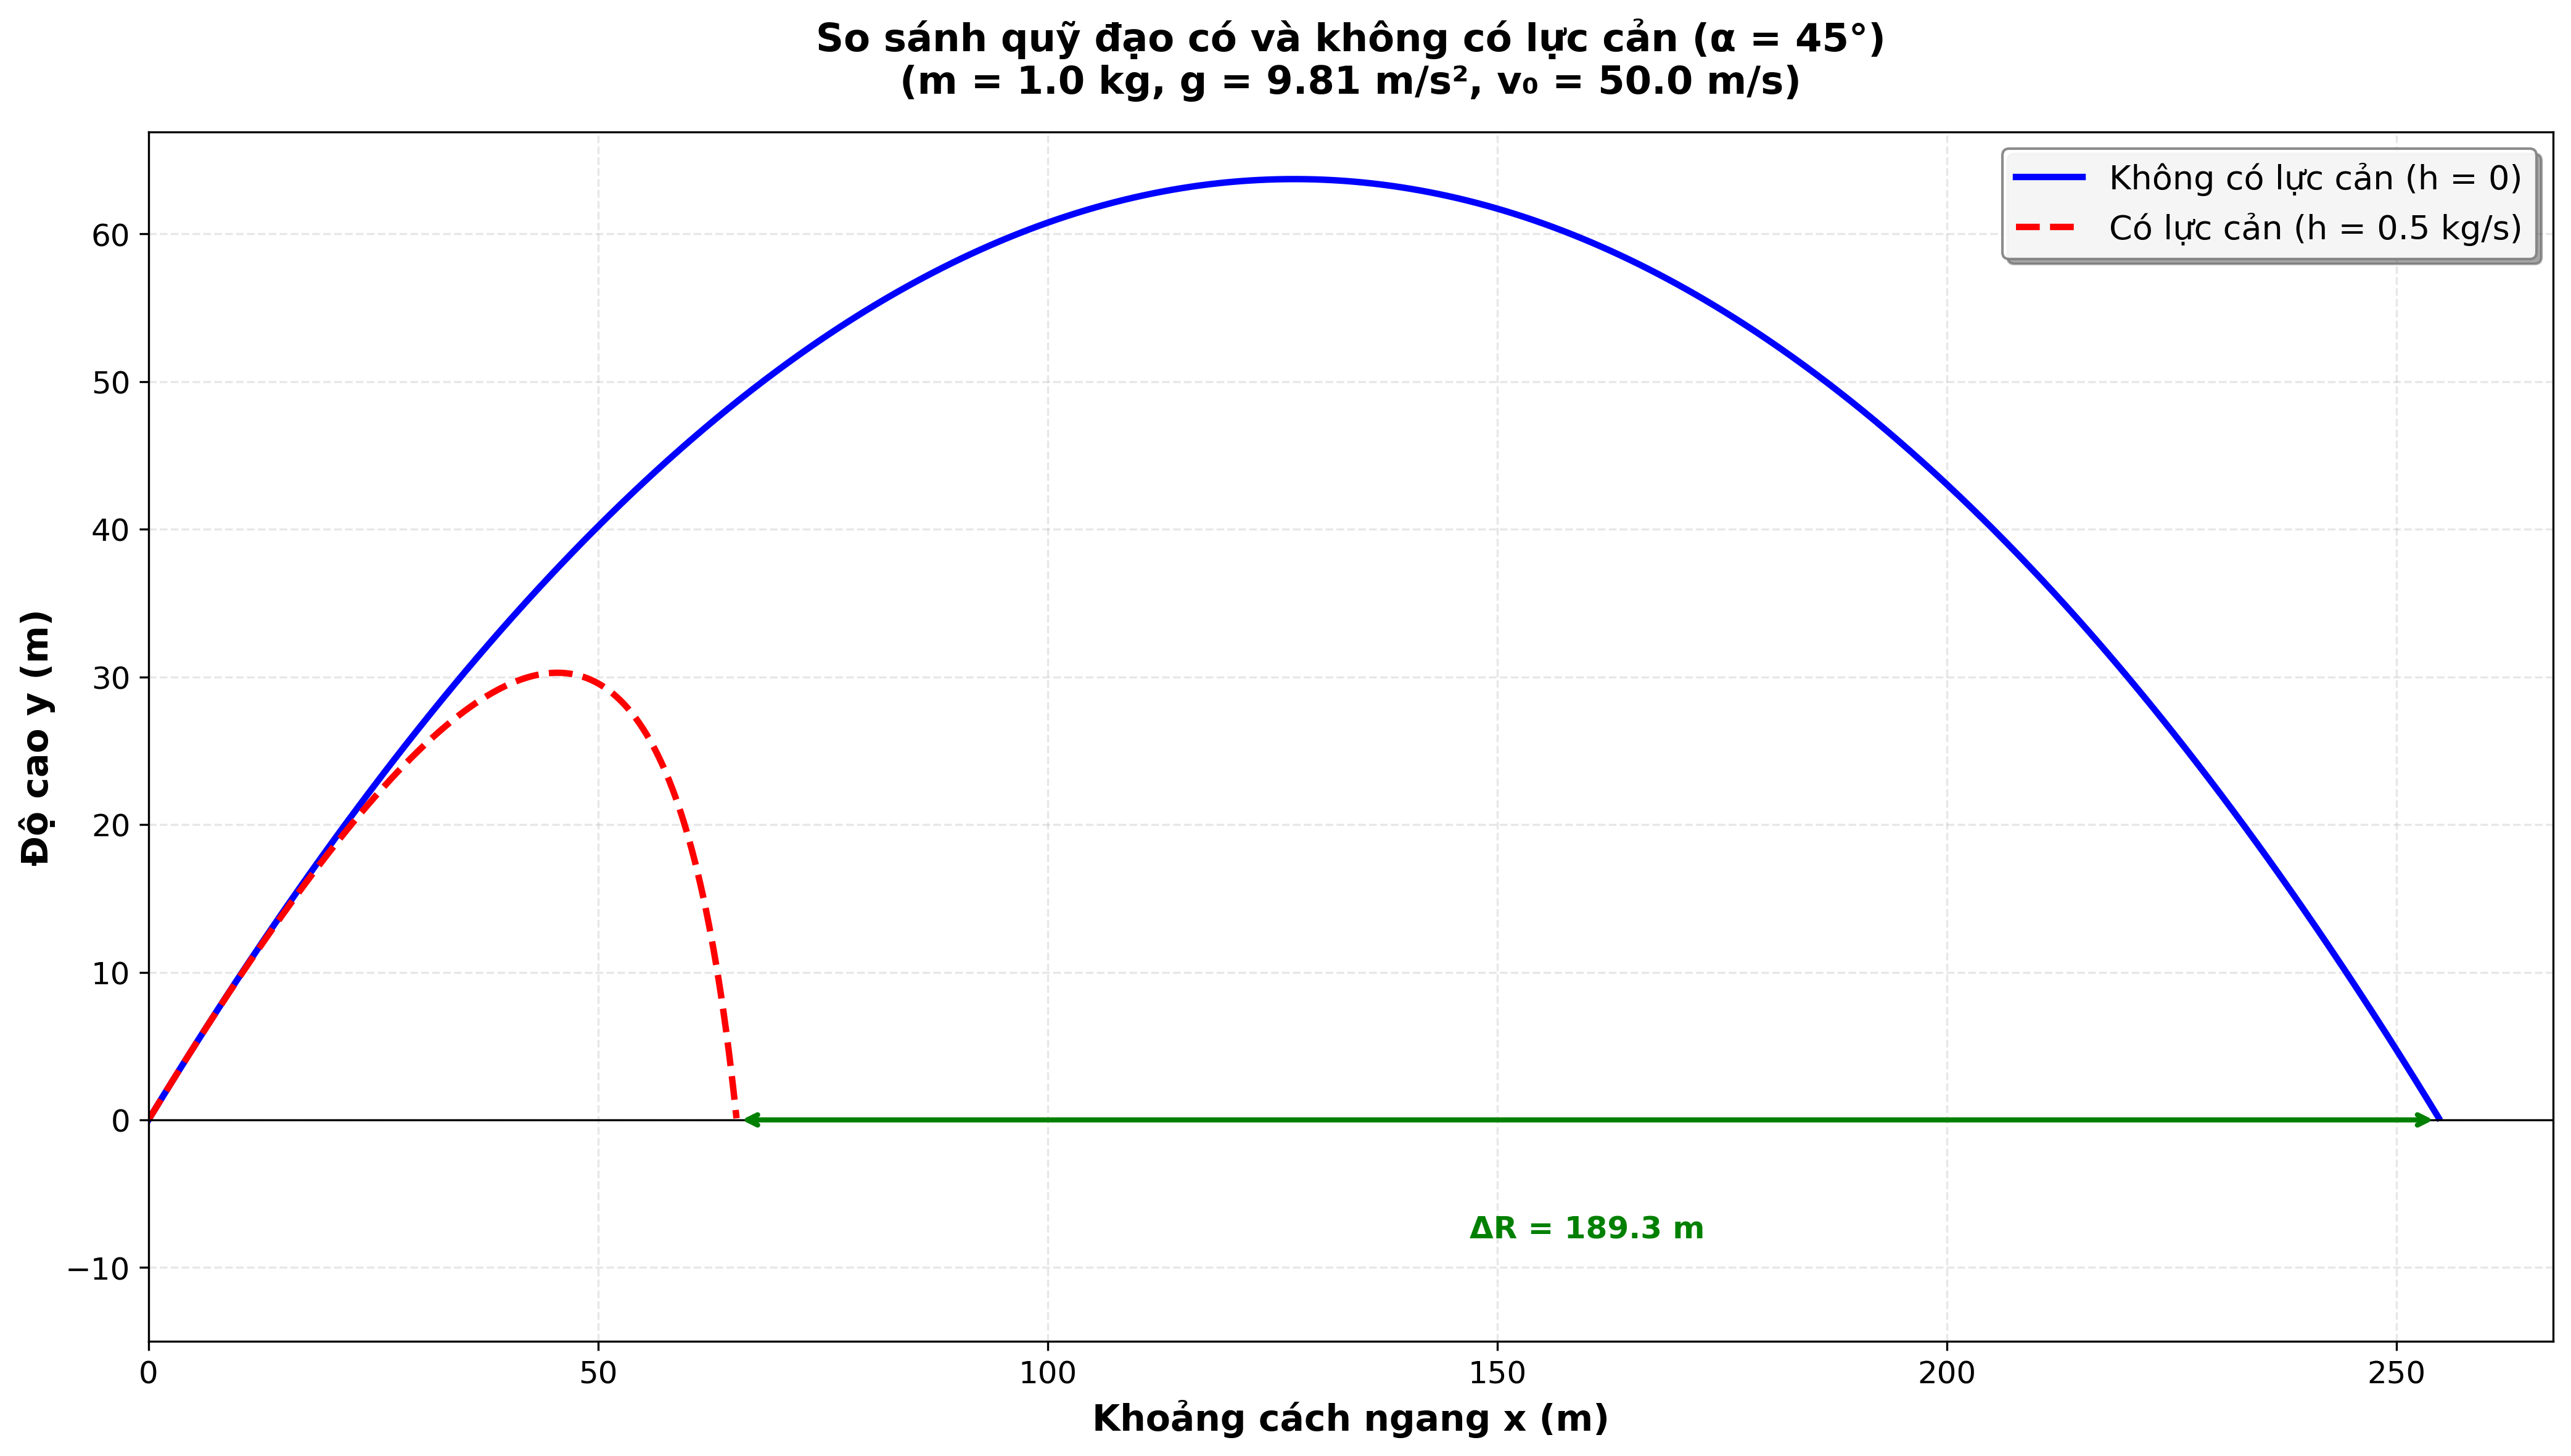
\includegraphics[width=\textwidth]{images/so_sanh_luc_can.png}
\caption{So sánh đường bay ở góc 45°: đường liền (xanh) -- lý tưởng; đường nét đứt (đỏ) -- có lực cản $h = 0{,}5$ kg/s.}
\label{fig:comparison}
\end{figure}

Sự khác biệt là rất lớn:
\begin{itemize}[nosep]
    \item Tầm xa: Từ $\approx 255$ m tụt xuống chỉ còn $\approx 65$ m (mất đi $\sim$74\%).
    \item Độ cao tối đa: Từ $\approx 64$ m tụt xuống $\approx 30$ m (mất đi $\sim$53\%).
    \item Thời gian bay: Từ $\approx 7{,}2$ s tụt xuống $\approx 5{,}2$ s.
\end{itemize}

Kết quả này cho thấy trong thực tế (như ném bóng, bắn súng, đánh golf...), lực cản của không khí đóng vai trò cực kỳ quan trọng. Nếu tính toán mà bỏ qua lực cản thì kết quả sẽ sai bét so với thực tế.


\subsection{Sự thay đổi của vận tốc}

\begin{figure}[H]
\centering
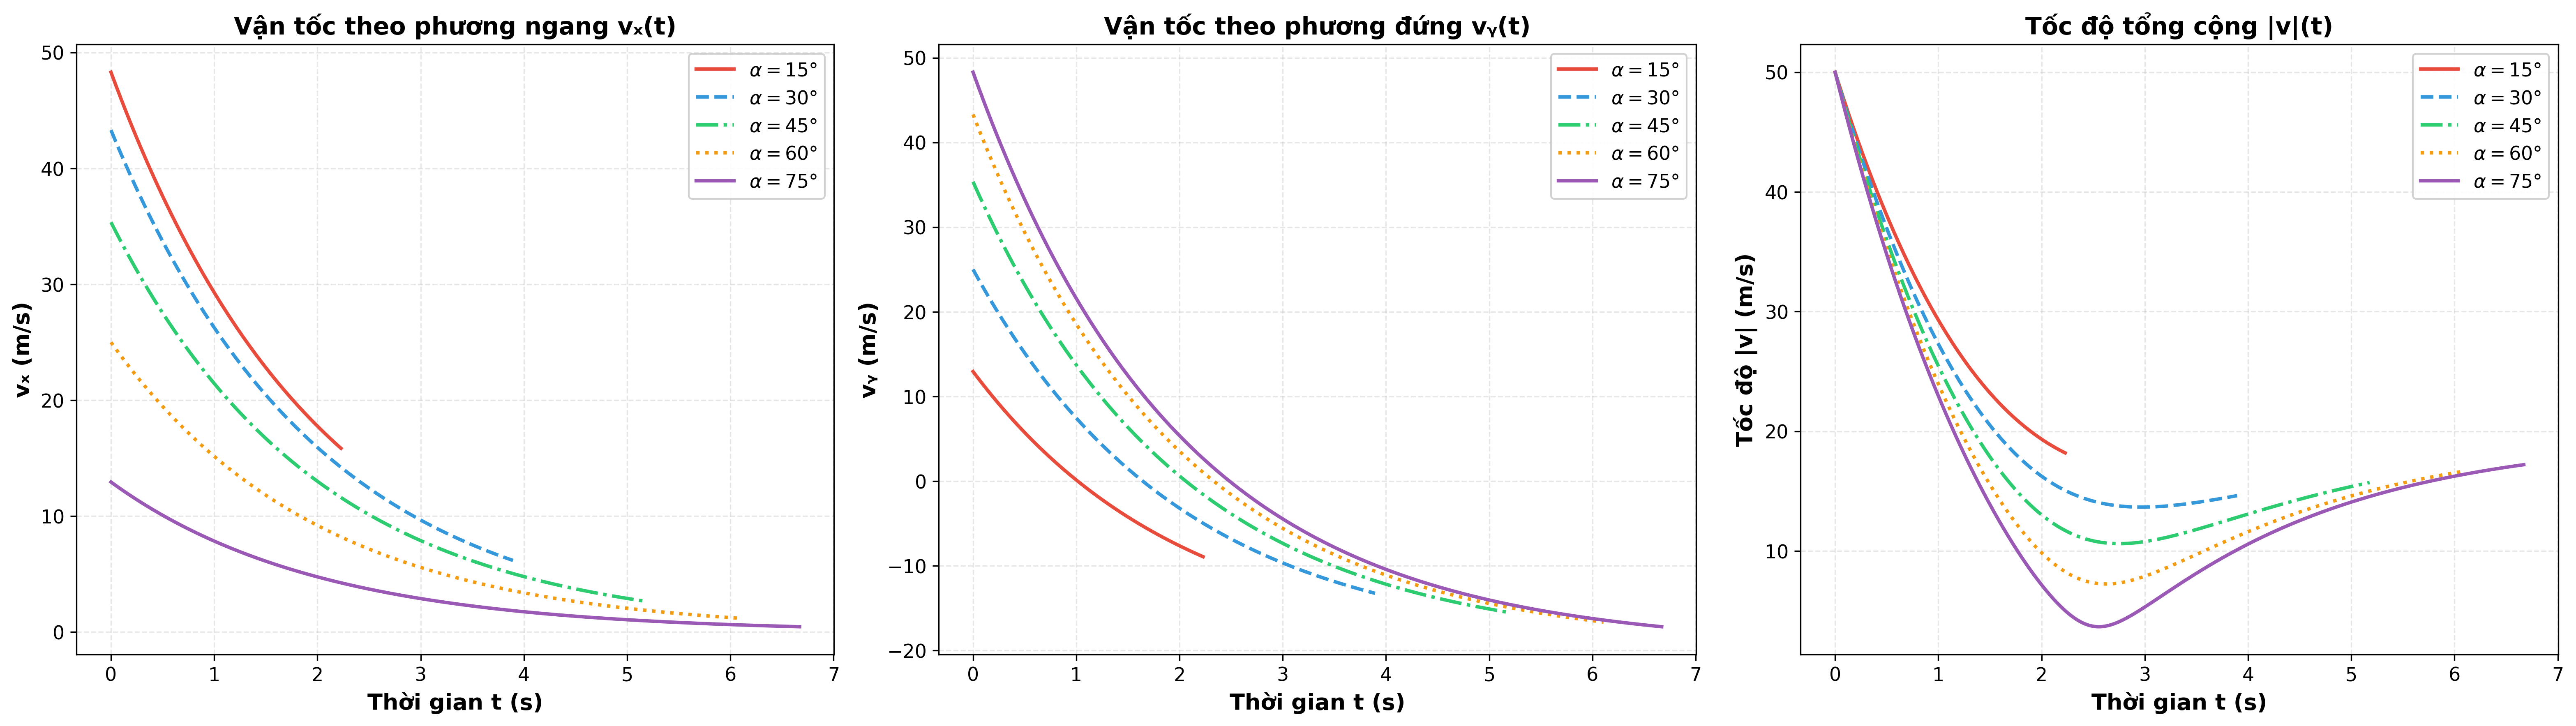
\includegraphics[width=\textwidth]{images/van_toc_theo_thoi_gian.png}
\caption{Đồ thị thay đổi vận tốc: ngang (trái), dọc (giữa), và tốc độ tổng cộng (phải) theo thời gian.}
\label{fig:velocity}
\end{figure}

Từ đồ thị Hình~\ref{fig:velocity}, ta thấy:

\begin{itemize}
    \item Vận tốc ngang (hình trái) cứ giảm dần đều và từ từ tiến về 0. Góc ném càng nhỏ (bay ngang nhiều) thì lực cản ngang càng mạnh nên tốc độ tụt càng nhanh.
    
    \item Vận tốc dọc (hình giữa) ban đầu giảm qua mức 0 (lúc vật đạt đỉnh), sau đó rơi xuống và kịch sàn ở mức $\approx -19{,}62$ m/s. Đây chính là "vận tốc giới hạn" mà ta đã nhắc ở phần lý thuyết. Vật không thể rơi nhanh hơn mức này được nữa.
    
    \item Tốc độ tổng cộng (hình phải) giảm nhanh lúc mới ném, nhưng đoạn sau chỉ hội tụ về đúng mức vận tốc giới hạn lúc rớt xuống chạm đất.
\end{itemize}


\subsection{Sự thay đổi năng lượng}

\begin{figure}[H]
\centering
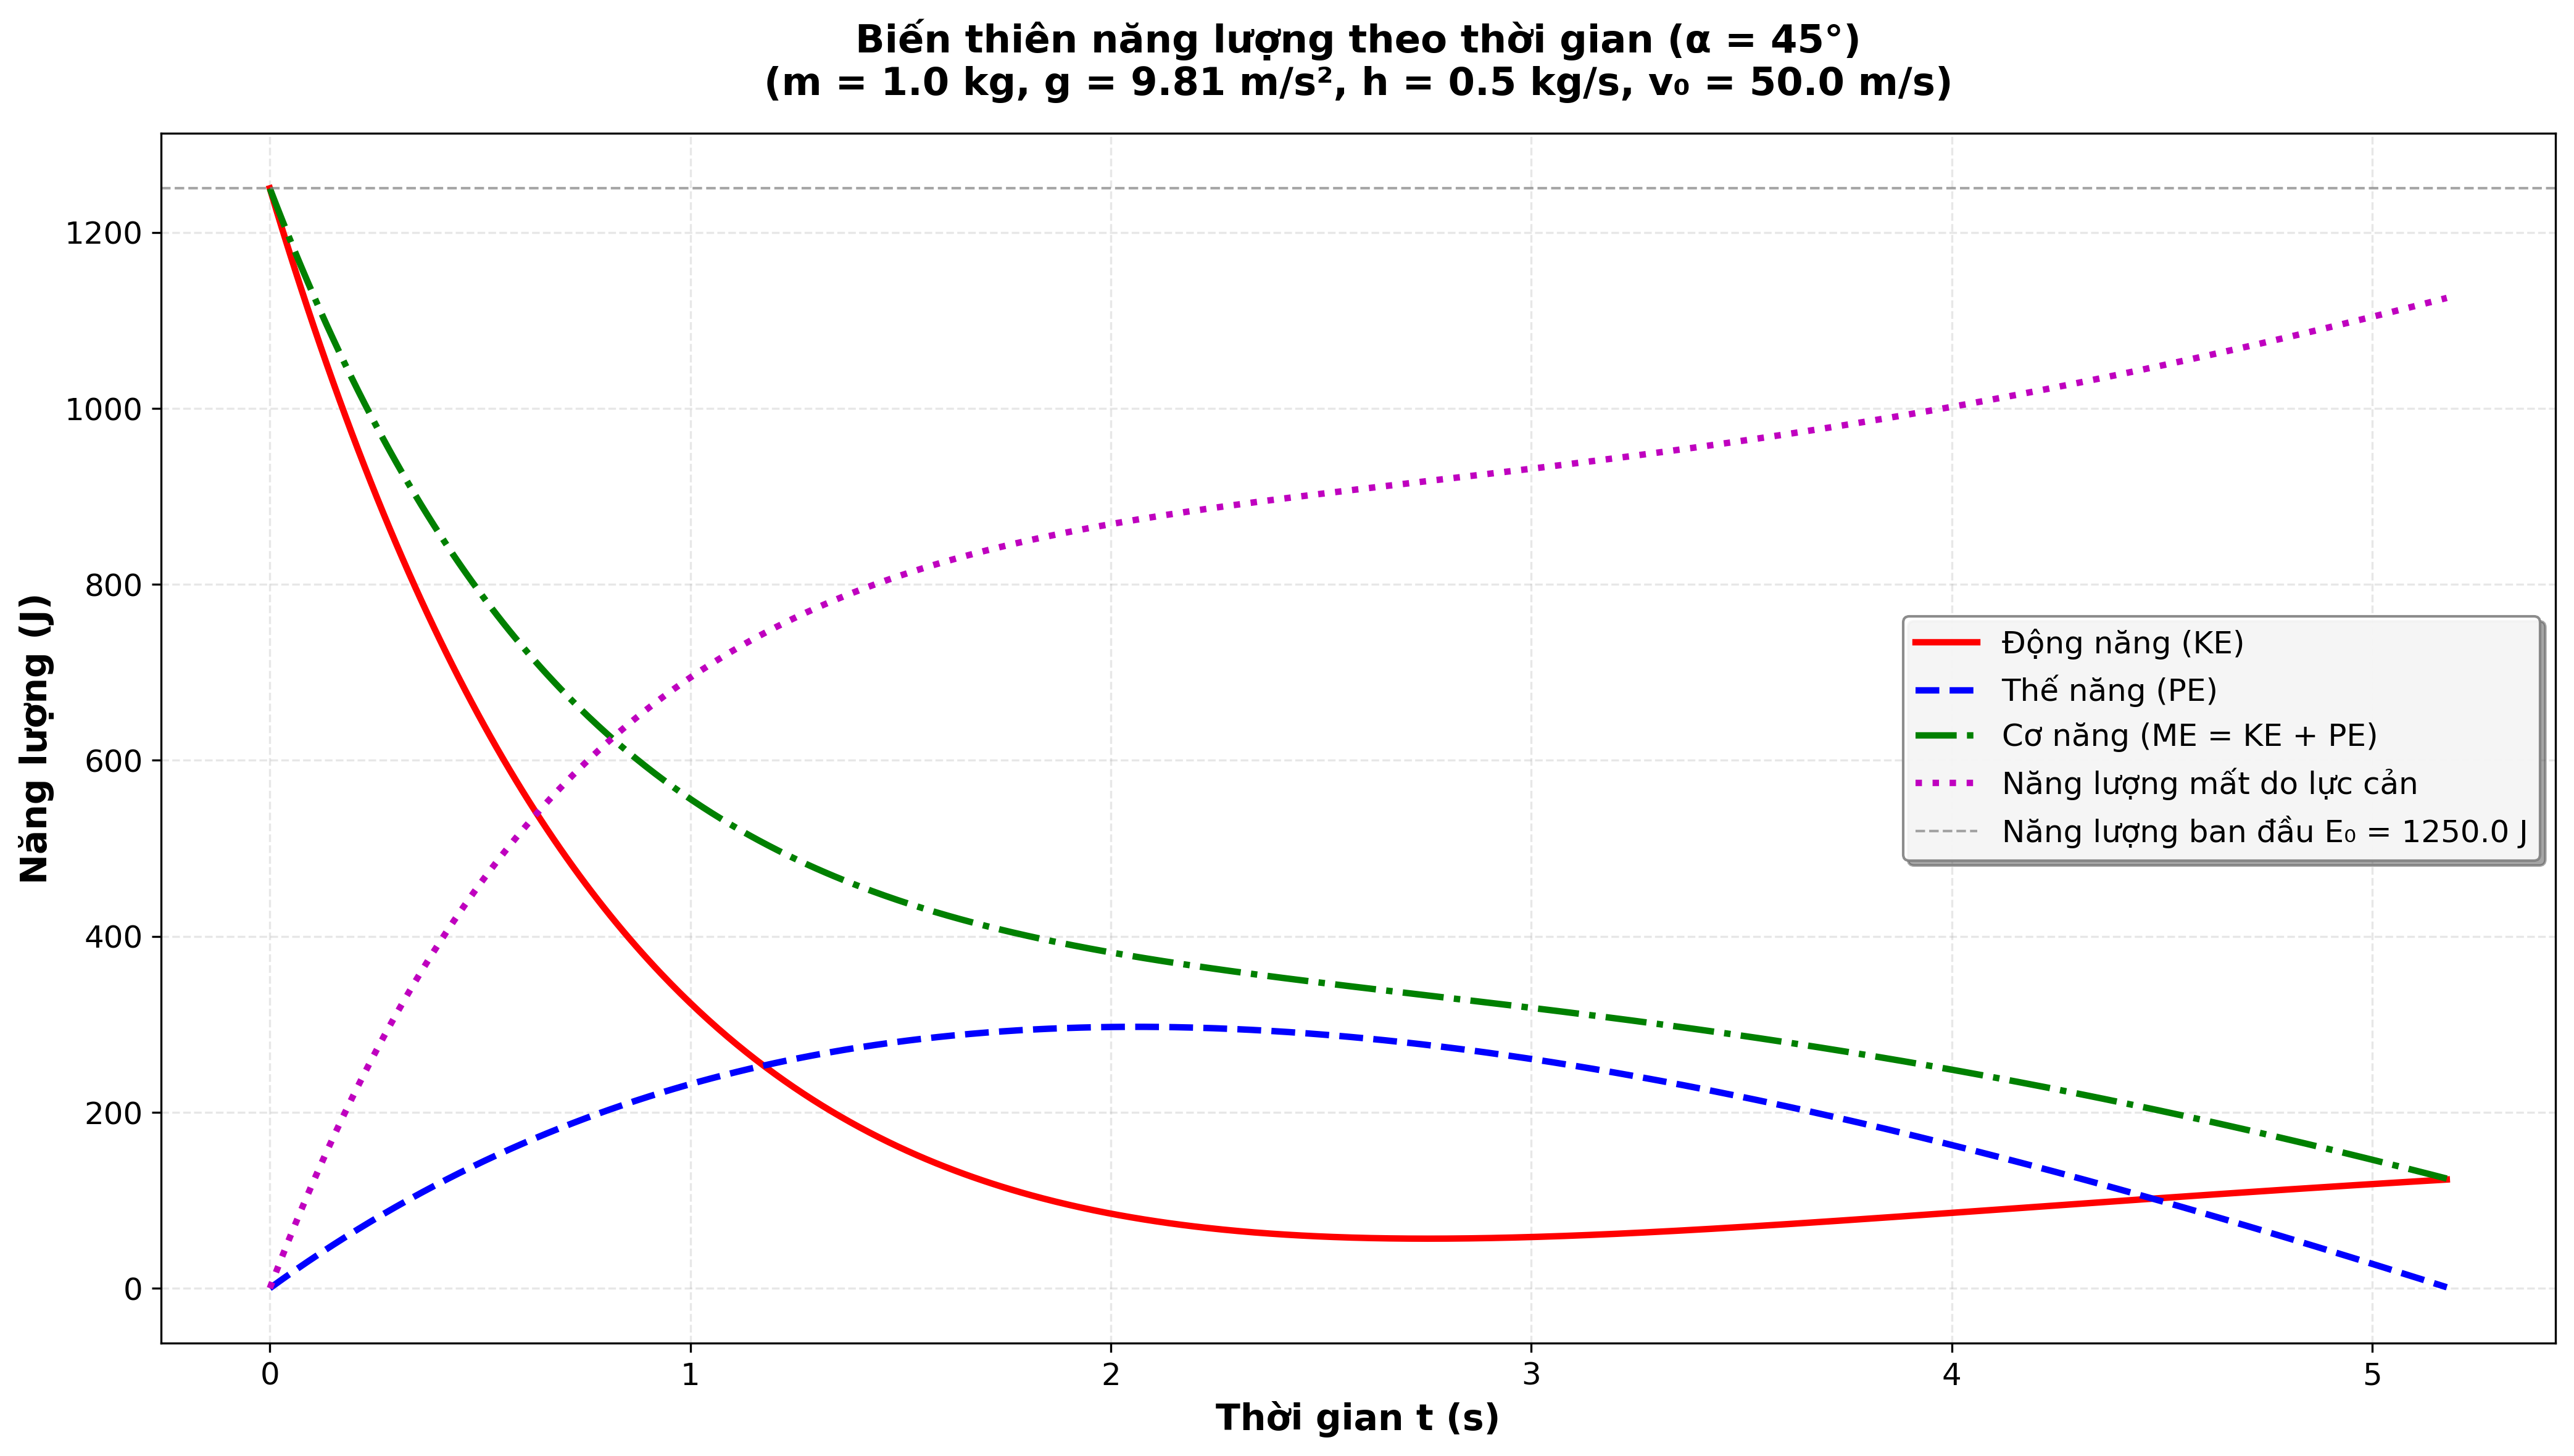
\includegraphics[width=\textwidth]{images/nang_luong_theo_thoi_gian.png}
\caption{Phân tích năng lượng khi ném ở góc 45°: động năng (đỏ), thế năng (xanh dương), cơ năng tổng (xanh lá), năng lượng mất đi (tím).}
\label{fig:energy}
\end{figure}

Nhìn vào đồ thị năng lượng (Hình~\ref{fig:energy}):

\begin{itemize}
    \item \textbf{Động năng} tụt rất nhanh lúc mới ném ra (vì vật bay nhanh, lực cản lớn).
    \item \textbf{Thế năng} tăng lên lúc bay lên đỉnh rồi giảm về 0 lúc rớt xuống đất.
    \item \textbf{Cơ năng} (tổng của động năng và thế năng) cứ giảm liên tục. Năng lượng này không tự nhiên sinh ra hay mất đi, mà nó đã chuyển hóa thành nhiệt năng do ma sát với không khí (phần năng lượng bị mất - đường màu tím).
    \item Đáng chú ý là khi vật vừa chạm đất, khoảng 85--87\% năng lượng ban đầu người ném truyền cho vật đã bị không khí hấp thụ hết.
\end{itemize}


\subsection{Hệ số cản mạnh yếu khác nhau thì sao?}

\begin{figure}[H]
\centering
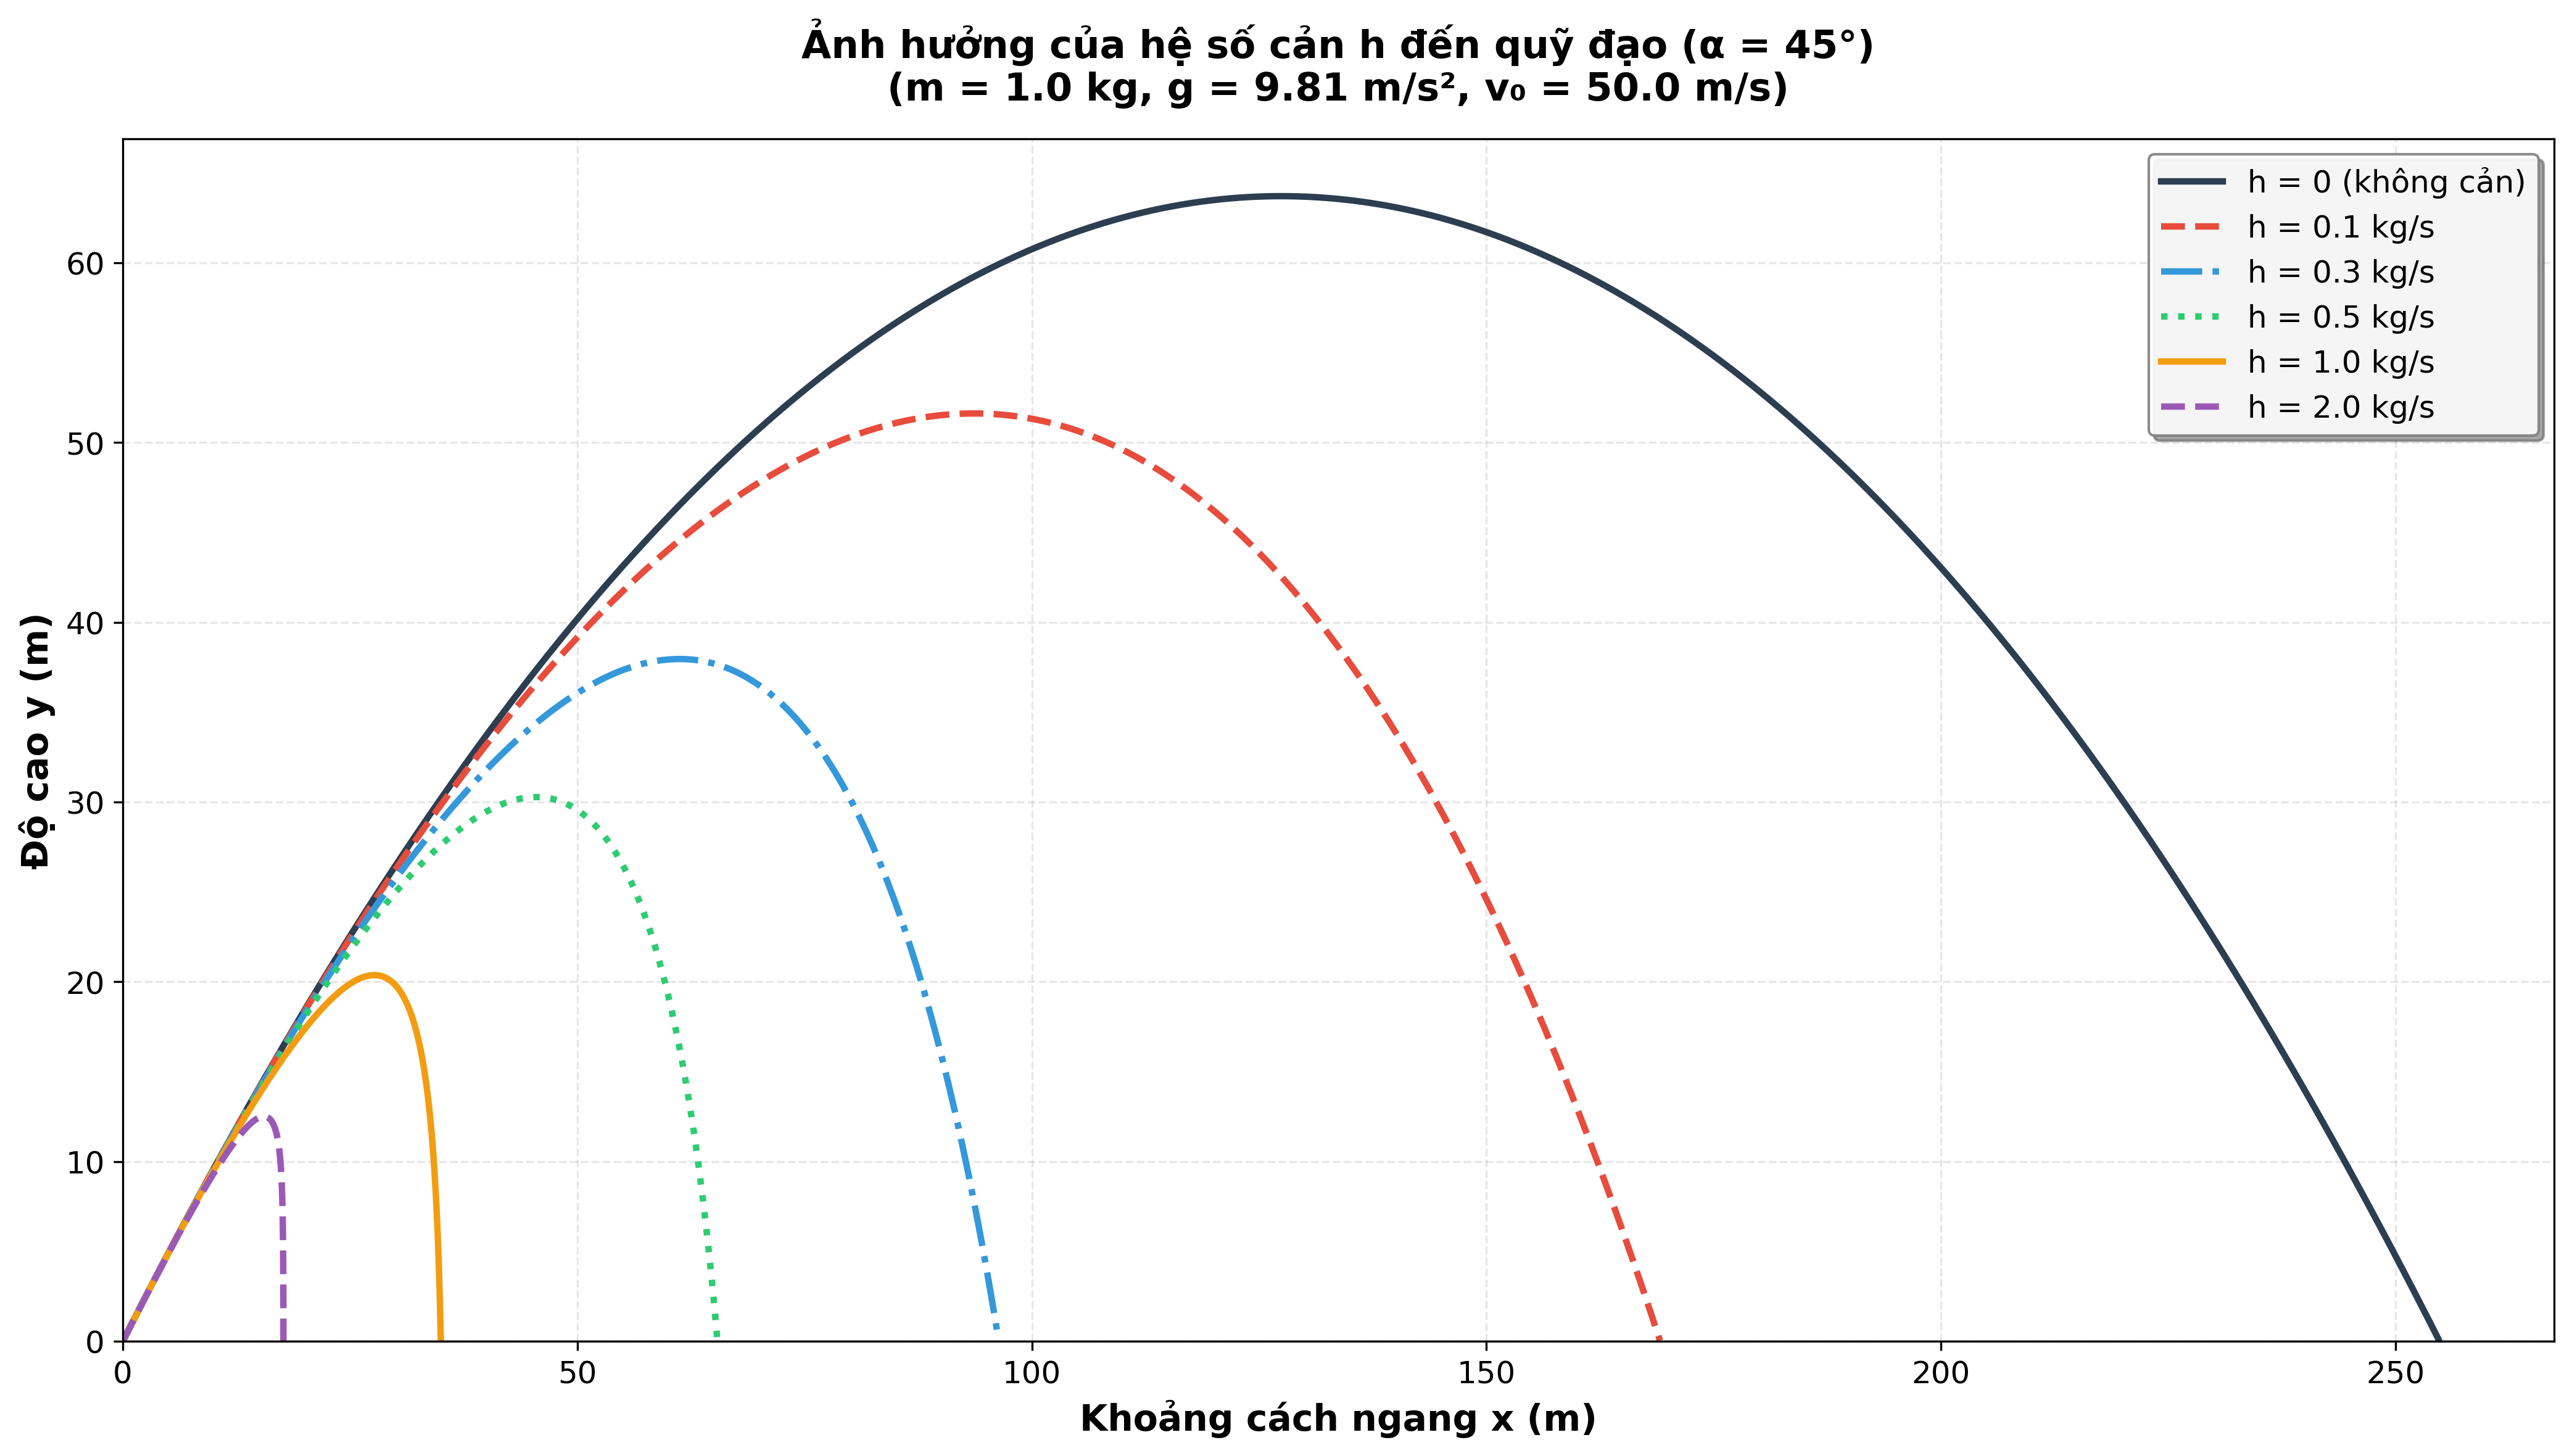
\includegraphics[width=\textwidth]{images/anh_huong_he_so_can.png}
\caption{Đường bay bị "móp" lại khi tăng dần lực cản $h$ từ 0 đến 2{,}0 kg/s (ném ở góc 45°).}
\label{fig:drag_effect}
\end{figure}

Hình~\ref{fig:drag_effect} cho ta thấy sức mạnh của lực cản:

\begin{itemize}
    \item Khi $h = 0$: đường bay đẹp, đối xứng hoàn hảo.
    \item Khi $h$ nhích lên một chút ($h = 0{,}5$), đường bay bị móp lại rõ rệt, rớt rất gần.
    \item Tuy nhiên, khi lực cản tiếp tục tăng (lên $1{,}0$ rồi $2{,}0$), sự khác biệt không còn quá sốc như lúc từ 0 lên $0{,}5$ nữa. Lý do là vì không khí cản quá mạnh khiến vật bay chậm rì, mà vật bay chậm thì lực cản lại yếu đi, tạo ra một trạng thái cân bằng.
    \item Nếu $h = 2{,}0$ kg/s, vật bay như bị hãm lại, rớt cách người ném có $\approx 17$ m (chỉ bằng một phần nhỏ xíu so với lúc không có không khí).
\end{itemize}
